\section{Computation units}

Compuation units aka octa-nodes are the primary component in the Octa.Space infrastructure.
They are responsible for providing the compuation power for tasks solving.
In general the octa-node is a computer with some amount of CPUs, GPUs, memory and disk space.
Each node can be used for computation or/and data storing and serving.
\\

It's necessary to install the special software on the computer to start accepting and solving the tasks.
This software is called \textbf{ORC}, it acts as a middleware between OS and compuation environments.
\\

\textbf{ORC} is responsible for the following:

\begin{itemize}
    \item Expose secure RPC channel to receive commands
    \item Organize isolated environments for the tasks
    \item Collect the system parameters, metrics and loads
    \item Provide the data storage interface
    \item Self-upgrade and self-maintenance operations
\end{itemize}

\begin{figure}[h]
\centering
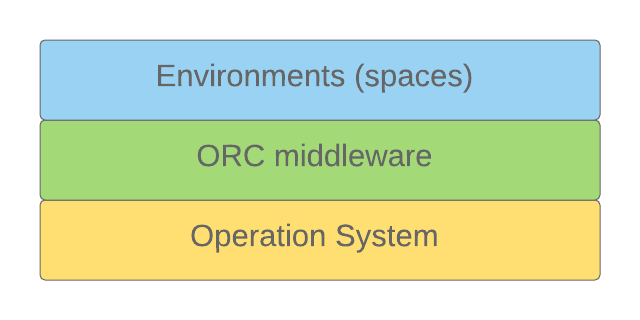
\includegraphics[width=5cm]{os-orc-spaces}
\caption{Octa-node layers}
\end{figure}

Secure channel is implemented using HTTPS\cite{https} protocol with each request validation using security token.

Security token is a fingerprint of the node, it's calculated in the following manner:

\begin{verbatim}
    Token = SHA256(IP, Timestamp, RandomInt)
\end{verbatim}

Where

\begin{itemize}
    \item IP - node public IPv4 address
    \item Timestamp - the time when node is installed in milliseconds
    \item RandomInt - random integer number
\end{itemize}

Commands recieved by the node are executed in the isolated environments.
These environments are called \textbf{spaces} and implemented using the Docker technology.

\newpage

\textbf{Spaces} is divided into two types: mandatory and task specific

\begin{figure}[h]
\centering
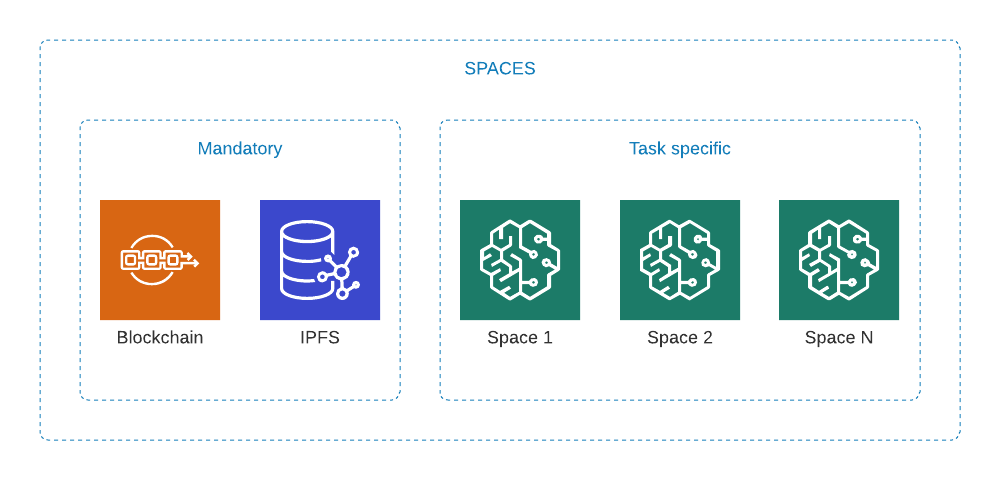
\includegraphics[width=10cm]{spaces}
\caption{Spaces}
\end{figure}

Mandatory \textbf{spaces} are always up and performs network maintainance and support functions.
Task specific \textbf{spaces} are run on-demand and depend on the type of the task which needs to be done.

System data are collected by \textbf{ORC}:

\begin{itemize}
    \item CPU information eg. amount, speed and utilization of cores
    \item GPU information including amount and model of GPUs, memory size and amount of graphic processors
    \item Total and free disk space, IO metrics
    \item Total and free memory amount
    \item Performance metrics like request-response time, network latency and so on
\end{itemize}

These data are used to improve the quality of the nodes and exclude the low performance nodes or non stable ones.

In cases when it's impossible to use IPFS for task data \textbf{ORC} internal storage will be used.
